\documentclass[sigconf]{acmart}
\usepackage{amsthm}
\usepackage{enumitem}
\usepackage{fancyhdr} 
\usepackage{graphicx}
\usepackage{multirow}
\usepackage{subcaption}
\usepackage{soul}
\usepackage{url}
\usepackage{xcolor}

\usepackage[linesnumbered,algoruled,boxed,lined,noend]{algorithm2e}

\newcommand{\spara}[1]{\smallskip\noindent{\bf #1}}

\newtheorem{problemDefinition}{Problem definition}
\newtheorem{definition}{Definition}
\newtheorem{property}{Property}
\newtheorem{lemma}{Lemma}
\newtheorem{strategy}{Strategy}
\newtheorem{corollary}{Corollary}
\newtheorem{example}{Example}
\newtheorem{theorem}{Theorem}

\DeclareMathOperator*{\argmax}{arg\,max}
\DeclareMathOperator*{\argmin}{arg\,min}

\newcommand{\BK}{\textsf{BK}}
\newcommand{\flexi}{\textsf{Flexi$-$clique}}
\newcommand{\KT}{\textsf{KT}}
\newcommand{\BRK}{\textsf{BK}}
\newcommand{\GW}{\textsf{GW}}
\newcommand{\DB}{\textsf{DB}}
\newcommand{\AZ}{\textsf{AZ}}
\newcommand{\PB}{\textsf{PB}}
\newcommand{\LJ}{\textsf{LJ}}

\newcommand{\NPA}{\textsf{NPA}}
\newcommand{\DPA}{\textsf{DPA}}
\newcommand{\jh}[1]{{\color{blue}{\sf [Jung: #1]}}}

\AtBeginDocument{%
  \providecommand\BibTeX{{%
    Bib\TeX}}}


\begin{document}

\title{Flexi-clique: Exploring Flexible and Sub-linear Clique Structures}


\settopmatter{authorsperrow=4,printacmref=false}

\setcopyright{none}

\author{Song Kim}
\affiliation{%
  \institution{Ulsan National Institute of Science \& Technology}
  \city{Ulsan}
  \country{South Korea}}
\email{song.kim@unist.ac.kr}



\author{Junghoon Kim}
\authornote{Corresponding author}
\affiliation{%
  \institution{Ulsan National Institute of Science \& Technology}
  \city{Ulsan}
  \country{South Korea}}
\email{junghoon.kim@unist.ac.kr}


\author{Susik Yoon}
\affiliation{%
  \institution{Korea University}
  \city{Seoul}
  \country{South Korea}}
\email{susik@korea.ac.kr}


\author{Jungeun Kim}
\affiliation{%
  \institution{Inha University}
  \city{Incheon}
  \country{South Korea}}
\email{jekim@inha.ac.kr}



\renewcommand{\shortauthors}{Song Kim, Junghoon Kim, Susik Yoon, \& Jungeun Kim}


\begin{abstract}
Identifying cohesive subgraphs within networks is a fundamental problem in graph theory, relevant to various domains. The traditional clique problem, which finds fully connected subgraphs, often faces limitations due to its strict connectivity requirements. This paper introduces a novel degree-based relaxation model called {\flexi}, where the degree constraint is adjusted sub-linearly based on the subgraph size. We establish that the maximum {\flexi} problem is NP-hard and propose an efficient and effective peeling algorithm to address it. Our extensive experimental evaluation of real-world datasets demonstrates the effectiveness and efficiency of our approach in discovering large, cohesive subgraphs in networks.
\end{abstract}


\maketitle





\section{Introduction}
How can we identify the structure with the high cohesiveness in a network? The clique problem~\cite{luce1949method} provides an answer to this question. Given a simple and undirected graph, a clique is defined as a set of nodes within a graph, every two of which are connected. The unique characteristic of cliques serves as an effective and powerful tool to find tightly-knit subgraphs within various networks. Thus, it has gained significant interest and has been utilised in numerous applications such as graph clustering~\cite{schaeffer2007graph}, economics~\cite{boginski2006mining}, coding theory~\cite{etzion1998greedy}, scheduling~\cite{dorndorf2008modelling}, and bioinformatics~\cite{day1986computational}.


While the structure of a clique has practical implications, the criteria for identifying one are quite strict, requiring connections between every pair of nodes. In practice, therefore, it is known that the size of the maximum clique is relatively small even in very large graphs~\cite{leskovec2020mining, chang2019efficient}. In sociology, it is understood that as the size of a community grows, the connectivity between individuals tends to weaken, but the influence of a community becomes more pronounced~\cite{simmel1950sociology}. This concept leads to active discussions about exploring relaxed clique structures, especially with large subgraphs.

Several models mitigate clique constraints. The $s$-clique~\cite{luce1950connectivity} allows nodes within distance $s$ as neighbours. The $s$-club~\cite{mokken1979cliques} focuses on the maximum distance between nodes within the subgraph. The quasi-clique~\cite{abello2002massive} specifies a threshold for minimum density. The $k$-plex~\cite{seidman1978graph} allows a specified number of missing connections, useful for real-world networks where perfect cliques are rare. 

\begin{figure}[t]
\centering
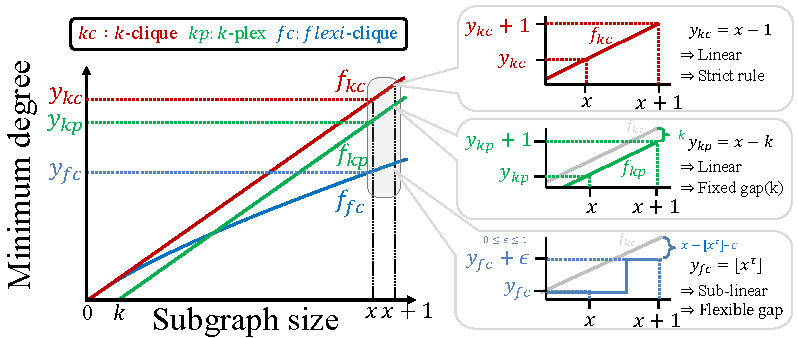
\includegraphics[width=0.9\linewidth]{figures/motivation_figure.pdf}
\vspace{-0.3cm} 
\caption{Motivation figure} 
\vspace{-1cm} 
\label{fig:motivation}
\end{figure}




While the $k$-plex has proven useful, its degree constraint increases linearly with the size of the subgraph which fundamentally limits the flexibility of approximation over varying sizes of the graph.
For smaller graphs, allowing $k$ disconnections within a subgraph can make the constraints overly relaxed. For larger graphs, on the other hand, it results in a similar strictness as cliques, making it difficult to find large $k$-plexes~\cite{miao2017approaches} when the subgraph size becomes very large. 


To address the issue of $k$-plex, we propose {\flexi}, a new degree-based relaxation model where the degree constraint is bounded by a given exponent regarding the subgraph size. This approach offers two main benefits: (1) \underline{\textit{flexibility}}: by allowing the degree constraint to adapt to the size of the subgraph, our model can capture meaningful subgraphs in networks with varying densities, and (2) \underline{\textit{sub-linearity}}: the minimum degree increases less strictly than linearly with the graph size, making it feasible to find larger cohesive subgraphs even in very huge networks.




Figure~\ref{fig:motivation} shows the differences between the $k$-clique, $k$-plex, and the {\flexi}. It demonstrates that $k$-clique, which is a clique with a size of $k$, demands a strict minimum degree proportional to the subgraph size. For $k$-plex, two aspects can be observed. Firstly, it does not produce  meaningful result until the subgraph size reaches $k$, meaning that when $k$ is large, it may ignore small subgraphs having dense structures. On the other hand, as the subgraph size increases, the minimum degree of $k$-plex also increases linearly. This implies that the strictness issue in $k$-clique could arise in the $k$-plex model as well when the subgraph size becomes bigger. 
%
However, {\flexi} has strict connectivity when the subgraph size is small but gradually relaxes the constraints as the subgraph size increases. This sub-linear adjustment allows the model to adapt more flexibly to different subgraph sizes, maintaining a balance between connectivity and flexibility. Consequently, {\flexi} can effectively identify larger, cohesive structures that other models might have missed.


In this paper, we study the maximum {\flexi} problem. Given a graph and a user-defined parameter, a {\flexi} is a connected subgraph where each node degree satisfies a sub-linear threshold relative to the subgraph size. The goal is to identify the largest subgraph satisfying these conditions. This problem is challenging due to the combinatorial nature of subgraph discovery and the dynamic adjustment of the degree constraint. We prove that the problem is NP-hard, propose an efficient peeling algorithm, and conduct extensive experiments on real-world networks to demonstrate the superiority of our proposed algorithm.



\spara{Contributions.} Our contributions are summarised as follows: (1) \underline{Novel relaxation model}: To the best of our knowledge, this work introduces the first sub-linear degree-based clique relaxation for the efficient discovery of cohesive subgraphs; (2)  \underline{Proving NP-hardness}: We theoretically prove the NP-hardness of the maximum {\flexi} problem; and (3)  \underline{Extensive experiments}: With real-world network datasets, we have conducted a comprehensive experimental study, demonstrating the efficiency of our peeling algorithms.




\begin{figure}[t]
\centering
\begin{subfigure}{.32\linewidth}
\centering
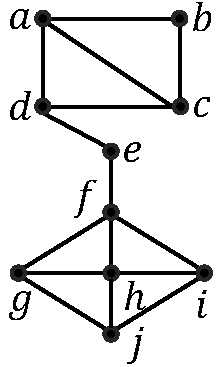
\includegraphics[width=0.7\linewidth]{figures/example_1.pdf}
\vspace{-0.2cm}
\caption{Input graph $G$}
\label{fig:graphs}
\end{subfigure}
\begin{subfigure}{.32\linewidth}
\centering
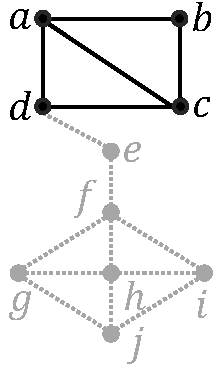
\includegraphics[width=0.7\linewidth]{figures/example_2.pdf}
\vspace{-0.2cm}
\caption{{\flexi}}
\label{fig:normal}
\end{subfigure}
\begin{subfigure}{.32\linewidth}
\centering
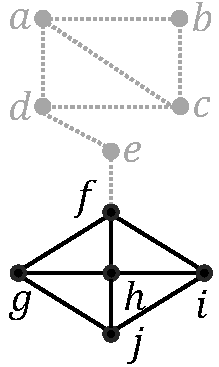
\includegraphics[width=0.7\linewidth]{figures/example_3.pdf}
\vspace{-0.2cm}
\caption{max. {\flexi} }
\label{fig:maximum}
\end{subfigure}
\vspace{-0.3cm}
\caption{{\flexi} example$(\tau =0.7)$}
\vspace{-0.45cm}
\label{fig:example}
\end{figure}


\section{Related Work}

Cohesive subgraph discovery is a fundamental problem in graph mining, with a wide range of applications in social network analysis, bioinformatics, and recommendation systems. Over the years, several models have been proposed to define and extract dense subgraphs, including cliques, quasi-cliques, and $k$-plexes. These models offer varying degrees of density and connectivity constraints, making them suitable for different use cases.

Clique is one of the earliest and most strict definitions of cohesive subgraphs. A clique is a subset of vertices in which every pair of vertices is connected by an edge. Given its strict requirement of complete connectivity, the maximum clique problem is known to be NP-hard~\cite{karp2010reducibility}. While cliques capture the most tightly connected structures in a graph, their strict definition often limits their applicability to small subgraphs in real-world networks.

To address this limitation, quasi-cliques~\cite{abello2002massive} were introduced as a relaxation of cliques, allowing some missing edges while still maintaining a high level of connectivity. Specifically, a quasi-clique ensures that a large proportion of possible edges exist within the subgraph. This relaxation increases the size of the subgraphs that can be discovered, making quasi-cliques useful in scenarios where perfect connectivity is not required.

Another popular relaxation model is the $k$-plex, which further generalises cliques by allowing each vertex to miss up to $k$ connections within the subgraph~\cite{seidman1978graph}. Formally, a $k$-plex of size $n$ is a subgraph where each vertex is adjacent to at least $n - k$ other vertices. This definition allows for significant flexibility, making $k$-plexes particularly useful for handling noisy or incomplete graphs, such as those encountered in biological networks.

Although various heuristic and exact algorithms have been proposed to discover cohesive subgraphs efficiently, existing models often struggle when applied to large networks. Their strict or unrealistic connectivity constraints can fail to capture flexible and meaningful substructures in real-world graphs. To address these challenges, we propose a novel model that balances subgraph size, density, and computational efficiency.


\section{Problem Statement}

In this work, let $G=(V, E)$ be a simple undirected graph, $G[S]$ the subgraph induced by $S \subseteq V$, $d(u, G)$ the degree of node $u$ in $G$, and $\delta(G)$ the minimum degree in $G$. We first formally define {\flexi}, then formulate the maximum {\flexi} problem.

\begin{definition}
(\underline{\flexi}.) Given a graph $G = (V, E)$ and a parameter $\tau$, a {\flexi}, denoted as $H$, is a node set such that:
\begin{itemize}
\item Every node $v \in H$ has at least $\lfloor |H|^\tau \rfloor$ degree in $G[H]$.
\item $G[H]$ is connected.
\end{itemize}
\end{definition}

\begin{problemDefinition}
(\underline{Maximum \flexi \, problem}.) Given a graph $G = (V, E)$ and a parameter $\tau$, the maximum {\flexi} problem is to find the largest {\flexi} of the given graph.
\end{problemDefinition}


\begin{example}
Given a graph $G$ in Figure~\ref{fig:graphs} with $\tau = 0.7$, the set of nodes ${a, b, c, d}$ forms a {\flexi} since it is connected and each node has at least $\lfloor 4^{0.7} \rfloor = 2$ neighbours. Similarly, the set of nodes ${f, g, h, i, j}$ also forms a {\flexi} as it satisfies the connectivity and degree constraints. This example shows that multiple {\flexi}s can exist within the same graph.
\end{example}


The maximum {\flexi} problem is challenging due to the combinatorial nature of subgraph discovery and the dynamic constraint on the minimum degree depending on the subgraph size. We now formally establish the computational hardness of this problem.

\begin{figure}[t]
\centering
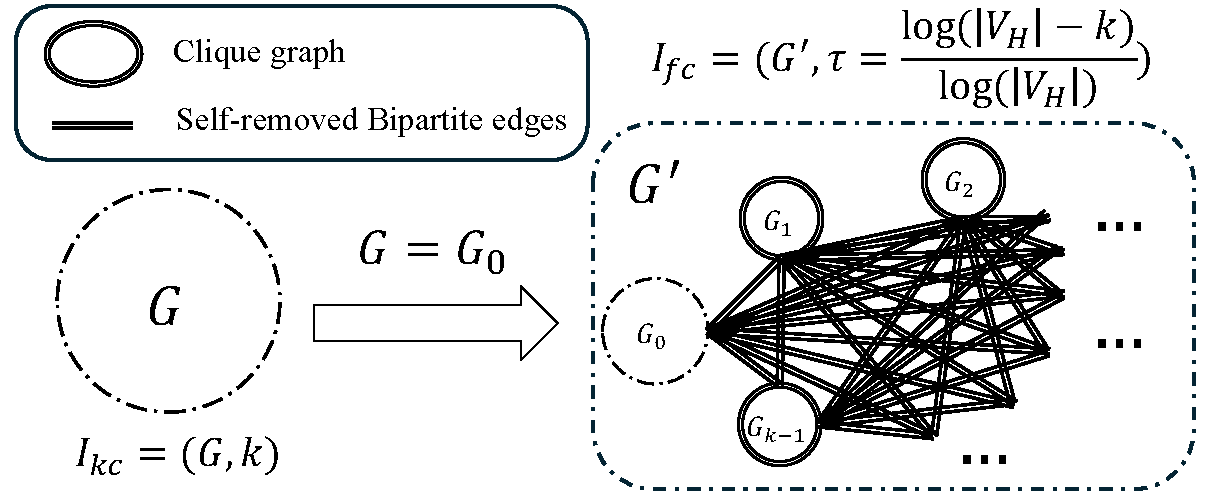
\includegraphics[width=0.9\linewidth]{figures/np-proof.pdf}
\vspace{-0.3cm} 
\caption{Reduction process} 
\vspace{-0.5cm} 
\label{fig:relax}
\end{figure}

\begin{theorem}
Maximum {\flexi} problem is NP-hard.
\end{theorem}
\vspace{-0.2cm}
\begin{proof}
To prove the NP-hardness of the maximum {\flexi} problem, we employ a novel reduction technique from the $k$-clique to $k$-plex~\cite{balasundaram2011clique} by incorporating an additional threshold $\tau$. Given a graph $G = (V, E)$ and an integer $k$, the decision version of the $k$-clique problem is to determine if there is a clique of size $k$. We denote an instance of the $k$-clique problem as $I_{kc} = (G, k)$. From the instance $I_{kc}$, we form an instance $I_{fc} = (G', \tau)$. In this instance, we aim to claim that identifying the maximum {\flexi} is at least as hard as finding a $k$-clique in $I_{kc}$. The graph generation and setting of the parameter $\tau$ are processed as follows. 

Formation from the instance $I_{kc}$ to $I_{fc}$ is presented in Figure~\ref{fig:relax}. First, we consider $G_0 = (V, E)$, which is the same as $G$ of $I_{kc}$ and we denote $n$ as $|V|$. Our newly generated graph $G'$ consists of $G_0, G_1, \ldots, G_{k-1}$. Note that for all $G_i$ where $1 \leq i \leq k-1$, each graph $G_i$ contains $n$ nodes and forms a clique, i.e., there are $\frac{n(n-1)}{2}$ edges in $G_i$. We call them clique graphs. In addition, any pair of graphs $G_x$ and $G_y$ where $x \neq y$ and $0 \leq x, y \leq k-1$ are connected by self-removed bipartite edges. The self-removed bipartite edges form a set of all edges from node $u \in V_x$ to $v \in V_y$ where $u \neq v$. Thus, each node $u \in V_x$ has $n-1$ connections to $V_y$.

Next, we set $\tau$ as $\frac{\log(|H|-k)}{\log(|H|)}$ where $|H|$ is a size of nodes of a connected subgraph $G[H]$:
\begin{align}
\lfloor |H|^{\frac{\log(|H|-k)}{\log(|H|)}} \rfloor \Rightarrow
\lfloor |H|^{\log_{|H|}(|H|-k)} \rfloor \Rightarrow |H|-k
\end{align}

Given an instance $I_{fc} = (G', \tau)$, we claim that the maximum {\flexi} is the set of nodes $H = C \cup V_1 \cup V_2 \cup \cdots \cup V_{k-1}$ where $C$ is a set of nodes in a clique of size $k$ in $G_0$. The size of $H$ is $n(k-1) + k$. Details in the degree of the nodes in $H$ are as follows:
\begin{itemize}[leftmargin=*]
\item Each node $v \in C$ has $k-1$ neighbours in $G_0[C]$ and $(n-1)(k-1)$ neighbours in clique graphs $G_1 \cup \cdots \cup G_{k-1}$.
\item Each node in clique graphs has at least $k-1$ neighbours in $G_0[C]$, $n-1$ neighbours in the same clique graph, and $(n-1)(k-2)$ neighbours in other clique graphs.
\end{itemize}

From this, we can find the relationship between the minimum degree of the nodes in $H$ and the size of $H$:
\begin{align}
\begin{aligned}
\delta(H) &= k-1 + (n-1)(k-1) = n(k-1) \\
&= n(k-1) + k - k = |H| - k
\end{aligned}
\end{align}

Therefore, it indicates that the identified nodes in $H$ satisfy the constraint of {\flexi}. This directly indicates that identifying {\flexi} in $I_{fc}$ is at least as hard as finding a $k$-clique in $I_{kc}$. Thus, {\flexi} is NP-hard.
\end{proof}





\section{Algorithm}

We present a non-articulation peeling algorithm ({\NPA}) to find the maximum {\flexi}. The high-level idea is to iteratively remove nodes while maintaining connectivity. For large graphs, the initial graph may require a high minimum degree. However, in real-world networks~\cite{clauset2009power, barabasi1999emergence}, many nodes have low degrees. Thus, we utilise $k$-core~\cite{seidman1983network}, a set of nodes where each has at least $k$ neighbours, to prune the nodes. The $k$-core can have multiple components, but we focus on the largest. Our empirical study shows that $k$-core returns few components, with the largest containing most nodes (Figure~\ref{fig:proportion}).

\begin{figure}[t]
\centering
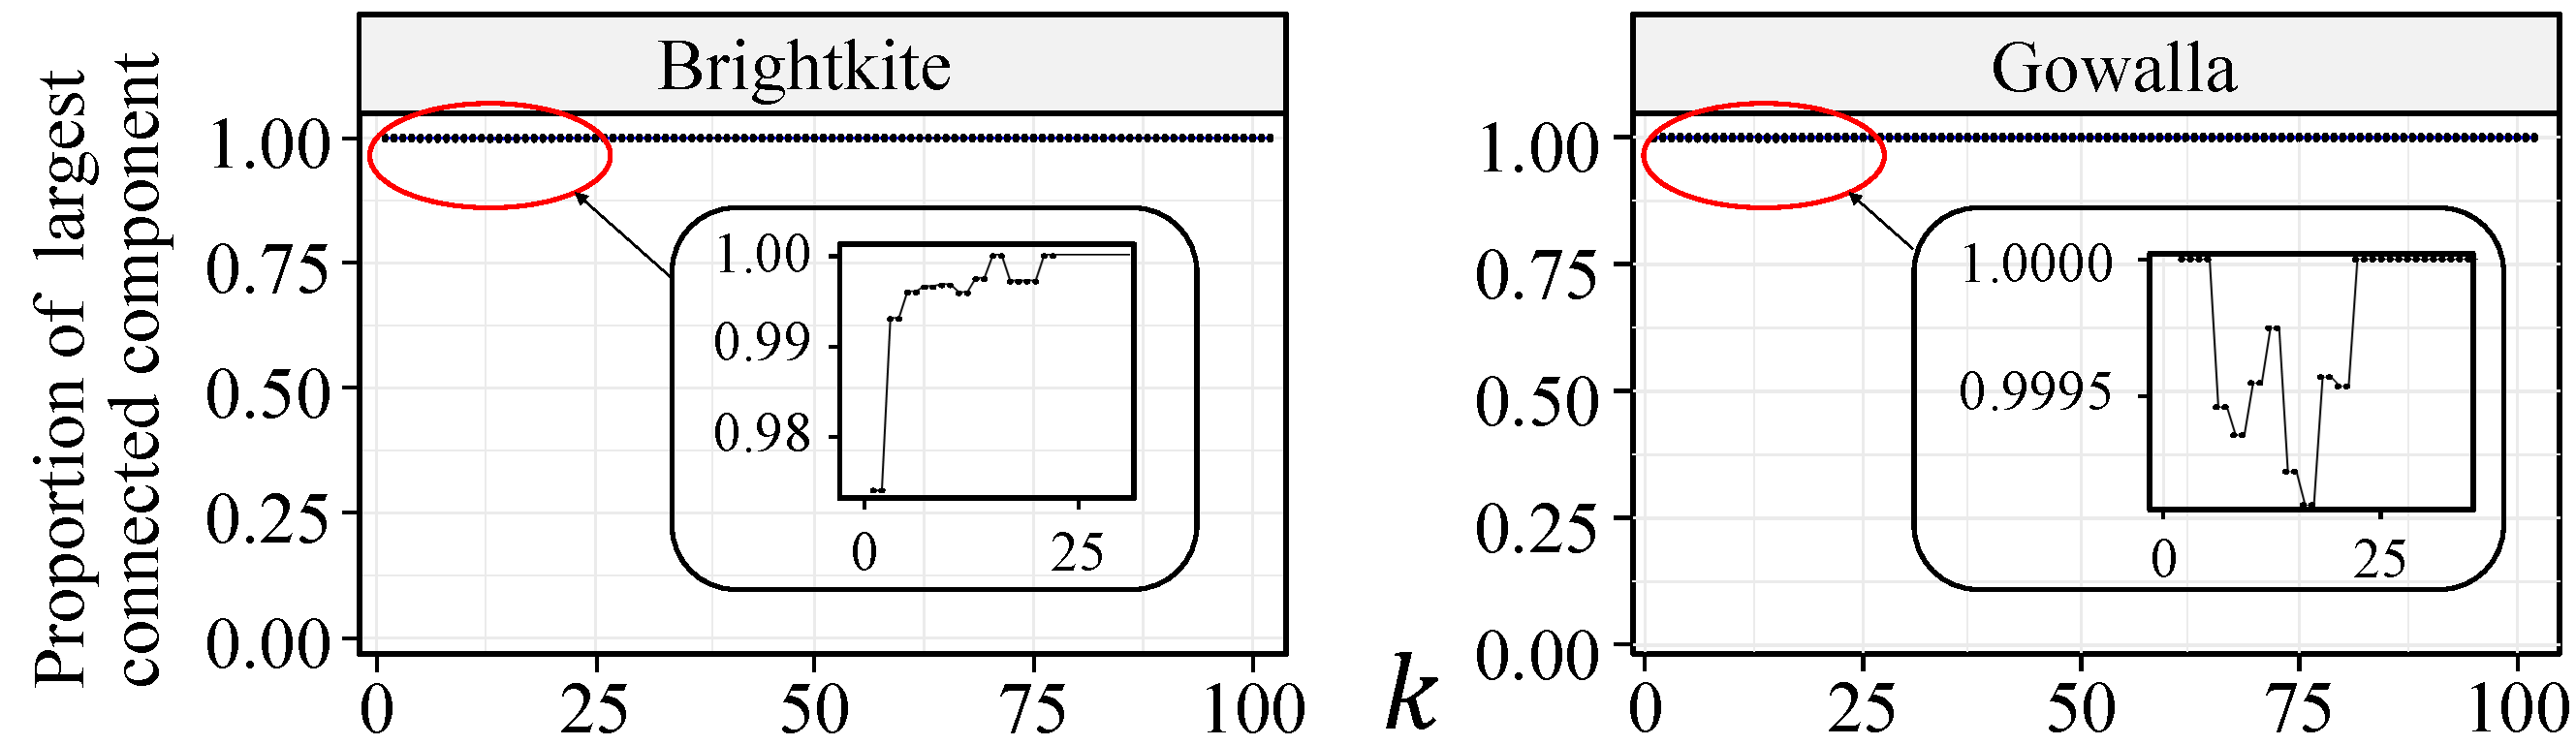
\includegraphics[width=0.85\linewidth]{figures/proportion_0.pdf}
\vspace{-0.3cm}
\caption{Proportion of the largest $k$-core component}  
\vspace{-0.35cm}
\label{fig:proportion}
\end{figure}

\spara{Algorithm description.} 
The pseudo description for the algorithm is presented in Algorithm~\ref{alg:peeling_t_clique1}. The {\NPA} increases $k'$ and finds all connected components for the $k'$-core. It stores all components, except the largest one, in a priority queue along with the current $k'$ value. If the largest connected component is a {\flexi}, it is added to the queue; otherwise, it is inserted into the priority queue (Lines 4-10). After traversing all possible $k$-cores, it iteratively retrieves subgraphs from the queue to build the initial graph for the peeling process. For each graph, non-articulation node with the minimum degree is iteratively removed while preserving the connectivity. If a {\flexi} is successfully found, the set of nodes in the subgraph is returned as the result (Lines 11-21). Otherwise, the next subgraph from the queue is processed. If the queue is empty, a subgraph is picked from the priority queue. This process is repeated until we identify a {\flexi}. Note that this approach puts a high priority on the largest connected component of each $k$-core to align with our objective function. 


\spara{Time complexity.} $O(k^* |V|\cdot(|V| + |E|))$ is the total time complexity of the {\NPA}. The complexities of the key components are as follows: 
\begin{itemize}[leftmargin=*] 
\item Coreness: Computing coreness of the nodes takes $O(|E|)$ time~\cite{batagelj2003m}. 
\item Finding connected components: Retrieving connected components takes $O(|V| + |E|)$ time, and this needs to be done $k^*$ times. 
\item Articulation nodes identification: This step can be performed in $O(|V| + |E|)$ time using a DFS-tree. 
\item Number of iteration: Given a specific subgraph, the number of iterations for the removal process is $O(|V|)$. 
\end{itemize}






\begin{algorithm}[t]
\small
\SetAlgoLined
\SetKwInOut{Input}{Input}
\SetKwInOut{Output}{Output}
\SetKw{return}{return}
\SetKw{OR}{OR}
\SetKw{break}{break}
\SetKwData{Comps}{Comps}
\SetKwData{PQ}{PQ}
\SetKwData{D}{D}
\SetKwData{c}{c}
\SetKwFunction{articulationNodes}{articulationNodes}
\SetKwFunction{max}{maxValue}
\SetKwFunction{push}{push}
\SetKwFunction{PriorityQueue}{PriorityQueue}
\SetKwFunction{pop}{pop}
\SetKwFunction{Queue}{Queue}
\SetKwFunction{addAll}{addAll}
\SetKwFunction{add}{add}
\SetKwFunction{coreness}{coreness}
\SetKwFunction{kcore}{kcore}
\SetKwFunction{kcoreCC}{kcoreCC}
\SetKwFunction{largestCC}{largestCC}
\SetKwFunction{connectedComp}{connectedComps}
\SetKwFunction{CC}{otherCC}
\Input{A graph $G = (V, E)$ and a threshold parameter $\tau$}
\Output{A {\flexi} $H$}
\BlankLine 
\c $\leftarrow$ \coreness{$G$} \tcp{Map storing coreness}
$PQ \leftarrow$ \PriorityQueue{} \tcp{Sort by size}
$Q \leftarrow$ \Queue{}, $T \leftarrow \emptyset$, $k^* \leftarrow$ \max{\c}\;
% $k' \leftarrow 2$\;
\For {($k' \leftarrow 2; k' \leq k^*; k'++$)}{
    $D \leftarrow$ \kcore{$k'$, \c}\;
    $C\leftarrow $ \connectedComp{$D$}\;
    $T \leftarrow \argmax_{t\in C} |t|$\;
    $PQ$.\add{$(t, k')$}, $\forall t\in C\setminus T$\;
    \lIf{$\lfloor|T|^\tau \rfloor \leq k'$}{
        $Q$.\add{$(T, k')$}
        %\break\;        
    } \lElse{
        $PQ$.\add{$(T, k')$}
    }
}
\While{$Q \neq \emptyset$ \OR $PQ \neq \emptyset$ }{
    \lIf {$Q \neq \emptyset$}{
        $T, k' \leftarrow Q$.\pop{}
    } \lElse{
        $T, k' \leftarrow PQ$.\pop{}
    }
    $k' \leftarrow k' - 1$\;
    $H\leftarrow$ \kcoreCC{$k'$, $T$, \c}\;
    \While{$\delta(H) < \lfloor |H|^\tau \rfloor$}{
        $A \leftarrow $\articulationNodes{$G[H]$}\;
        $T \leftarrow H \setminus A$\;
        $u \leftarrow \argmin_{v\in T} d(v, G[H])$\;
        $H \leftarrow H \setminus \{u\}$\;
    }
    \lIf{$H \neq \emptyset$}{
        \return $H$
    }
}
\return $\emptyset$\;
\caption{Peeling algorithm for the {\flexi} (\NPA)}
\label{alg:peeling_t_clique1}
\end{algorithm}


\begin{figure}[h]
\vspace{-0.3cm}
\centering
\begin{subfigure}{.32\linewidth}
\centering
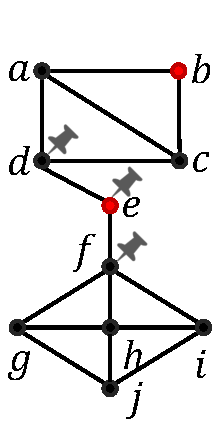
\includegraphics[width=0.7\linewidth]{figures/algorithm_1.pdf}
\vspace{-0.2cm}
\caption{Input graph $G$}
\label{fig:alg1}
\end{subfigure}
\begin{subfigure}{.32\linewidth}
\centering
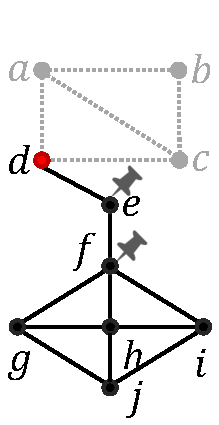
\includegraphics[width=0.7\linewidth]{figures/algorithm_2.pdf}
\vspace{-0.2cm}
\caption{Peeling process}
\label{fig:alg2}
\end{subfigure}
\begin{subfigure}{.32\linewidth}
\centering
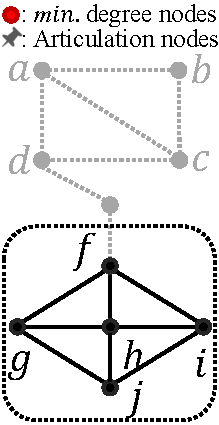
\includegraphics[width=0.7\linewidth]{figures/algorithm_3.pdf}
\vspace{-0.2cm}
\caption{Result}
\label{fig:alg3}
\end{subfigure}
\vspace{-0.3cm}
\caption{{\NPA} example}
\vspace{-0.3cm}
\label{fig:gpa}
\vspace{-0.3cm}
\end{figure}

\begin{example}
Using the graph in Figure~\ref{fig:example} with $\tau =$ $0.7$, we present the procedure of {\NPA} in Figure~\ref{fig:gpa}. Nodes with the minimum degree are marked in red and articulation nodes are marked as "pinned". The algorithm first finds the largest $k$-core component satisfying the {\flexi} constraint. Since the set $\{f, g, h, i, j\}$ forms both a $3$-core and a {\flexi}, the peeling process starts from the $2$-core containing the set, which is the whole graph. The algorithm iteratively checks and removes nodes not meeting the degree constraint while preserving connectivity. Thus, in Figure~\ref{fig:alg1}, node $e$ is not removed despite having the minimum degree. Figures~\ref{fig:alg2} and~\ref{fig:alg3} illustrate changes in articulation points during the process. Ultimately, the set $\{f, g, h, i, j\}$ is identified as the resultant {\flexi}.
\end{example}






\section{Experiments}

\subsection{Experimental setup.}
To evaluate the performance of our model and algorithm, we conduct an extensive experimental study. Through our experiments, we aim to address the following evaluation questions (\textbf{EQs}): (1) \textbf{ Effectiveness}: How accurately does our algorithm perform compared to the exact solution?; (2) \textbf{Effect on $\tau$}: How does varying $\tau$ impact resultant subgraphs? We  analyse the effects of different $\tau$ values on subgraph size; (3)  \textbf{Scalability}: How well does the proposed algorithm scale on datasets with different sizes?; and (4) \textbf{Effect on $k$-core.} How much does using $k$-core as a preprocessing step improve the running time of the peeling algorithm? 





\subsection{Experimental setting}
\begin{table}[t]
\small
\caption{Real-world datasets}
\vspace{-0.3cm}
\begin{tabular}{c||c|c|c}
\hline
\textbf{Dataset}    & \textbf{No. of nodes} & \textbf{No. of edges} & \textbf{No. of comm.} \\ \hline\hline
Karate (\KT)       & 34              &  78         & 2       \\ \hline \hline
% Polblogs (\PB)       & 1,224              &  16,718         & 2       \\ \hline
Brightkite (\BRK)  & 58,228          & 214,078     & -      \\ \hline  
Gowalla (\GW)      & 196,591         & 950,327     & -       \\ \hline
%DBLP (\DB)         & 317,080         & 1,049,866   & 13,477  \\ \hline
Amazon (\AZ)       & 334,863         & 925,827     & 75,149  \\ \hline \hline
\end{tabular}
\label{tab:dataset}
\vspace{-0.3cm}
\end{table}


\spara{Real-world datasets.}
Table~\ref{tab:dataset} provides the basic information of real-world datasets used in our experiments. These datasets are publicly available, as referenced~\cite{cho2011friendship,yang2012defining}. Note that Gowalla and Brightkite datasets have no ground-truth community information. 





\subsection{Experimental result}
\vspace{-0.3cm}
\begin{figure}[h]
\centering
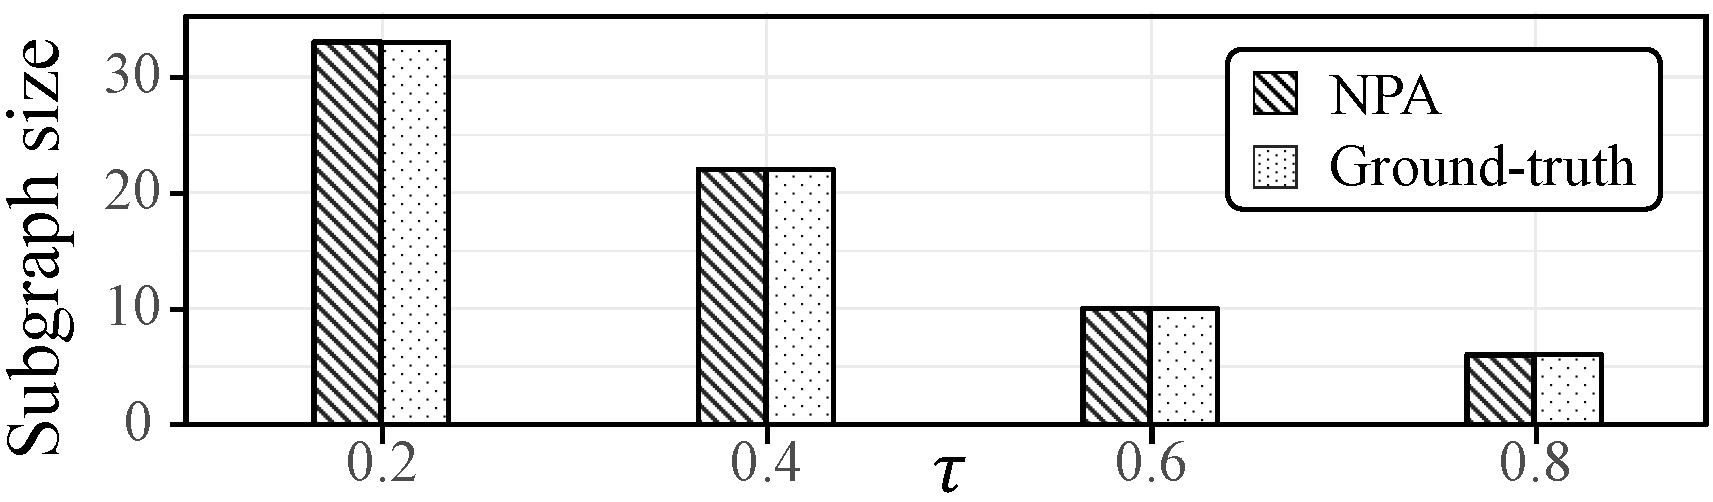
\includegraphics[width=0.8\linewidth]{figures/effect.pdf}
\vspace{-0.4cm}
\caption{\textbf{EQ1.} Comparing with Ground-truth}  
\vspace{-0.35cm}
\label{fig:ground_truth}
\end{figure}





\spara{\textbf{EQ1. Effectiveness}.} 
In this experiment, we compare the results of {\NPA} with the optimum solution obtained by enumerating all connected components in the small network(KT)~\cite{zachary1977information} using publicly available code~\cite{alokshiya2018linear}. Surprisingly, Figure~\ref{fig:ground_truth} shows that the proposed {\NPA} returned the same results as the optimum solution for all four different $\tau$ values tested. This remarkable consistency demonstrates the experimental effectiveness and robustness of our algorithm.

\begin{figure}[h]
\centering
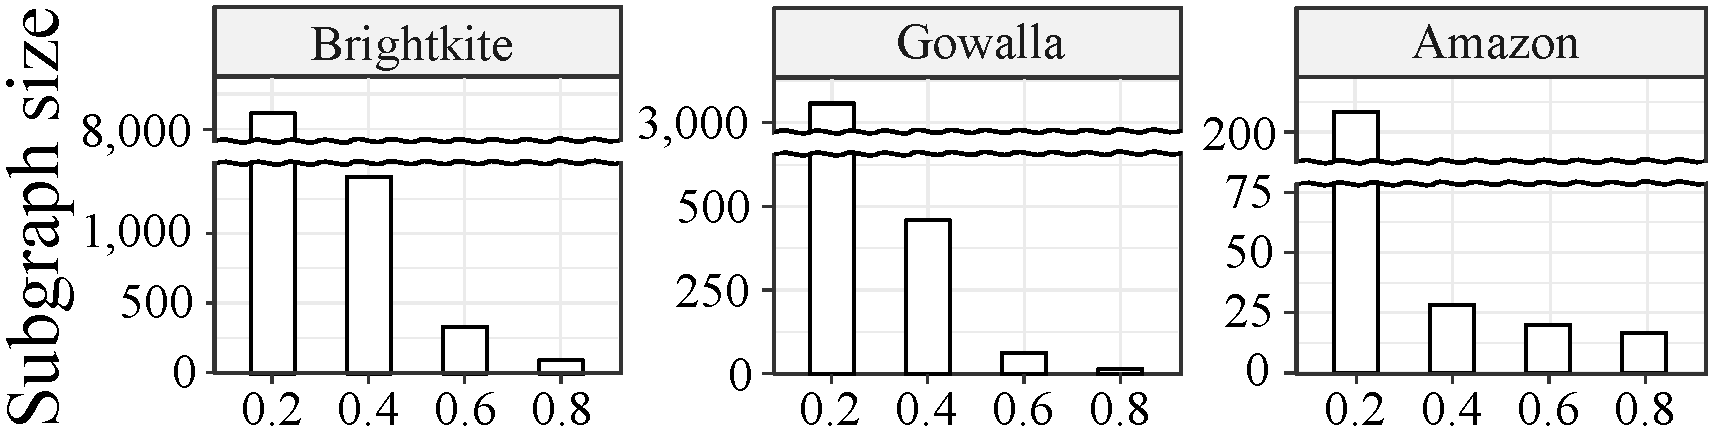
\includegraphics[width=0.8\linewidth]{figures/real_world.pdf}
\vspace{-0.3cm}
\caption{\textbf{EQ2.} Effect on $\tau$}  
\vspace{-0.35cm}
\label{fig:effect}
\end{figure}

\spara{\textbf{EQ2. Effect on $\tau$}.} We analyse how varying the $\tau$ of {\NPA} impacts the subgraph size. Figure~\ref{fig:effect} presents the results. As $\tau$ increases, the size of the {\flexi} consistently decreases because a larger $\tau$ indicates a search for a more cohesive subgraph structure. This increased cohesiveness requirement means that fewer nodes can satisfy the stricter connectivity, resulting in smaller subgraphs. 
\begin{figure}[h]
\centering
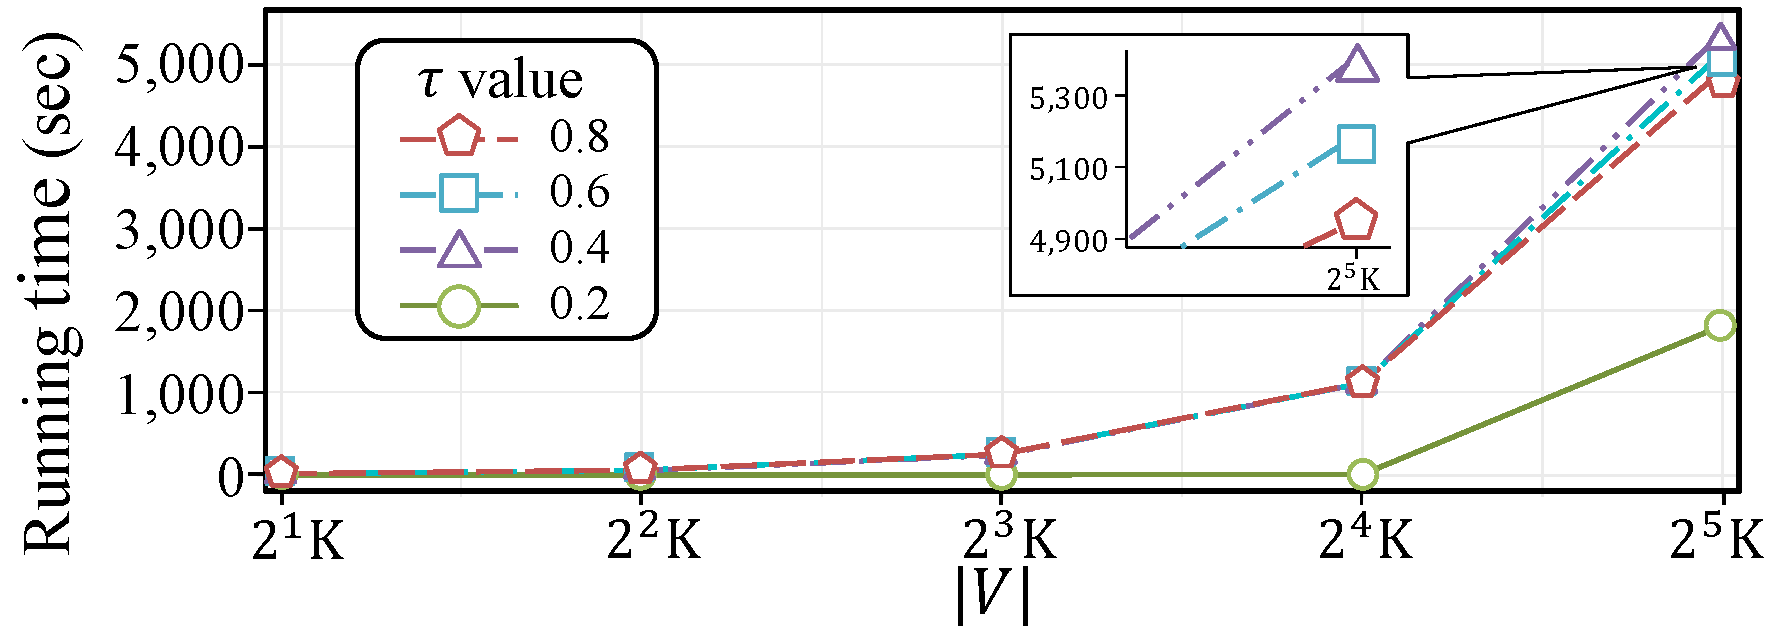
\includegraphics[width=0.9\linewidth]{figures/syn_time_log2_final.pdf}
\vspace{-0.3cm}
\caption{\textbf{EQ3.} Scalability test}  
\vspace{-0.4cm}
\label{fig:syn_time}
\end{figure}



\spara{\textbf{EQ3. Scalability test}.} We evaluate the scalability of our proposed algorithm on synthetic datasets~\cite{lancichinetti2008benchmark}. Using default parameters, we generate graphs varying in size from 2,000 to 32,000 nodes under different $\tau$ conditions. Figure~\ref{fig:syn_time} shows a near-linear increase in running time as the node size grows. Additionally, we observe that as $\tau$ increases, the running time does not consistently rise. 
%
This result can be explained as follows: For very small $\tau$ values, the nodes in the initial graph mostly satisfy the degree constraint early in the peeling process, requiring minimal iterations and resulting in a short running time. Conversely, for larger $\tau$ values, most nodes might be addressed during the preprocessing step which also leads to relatively short running time. Therefore, the algorithm takes the longest time for $\tau$ values that are neither too small nor too large.


\begin{figure}[h]
\centering
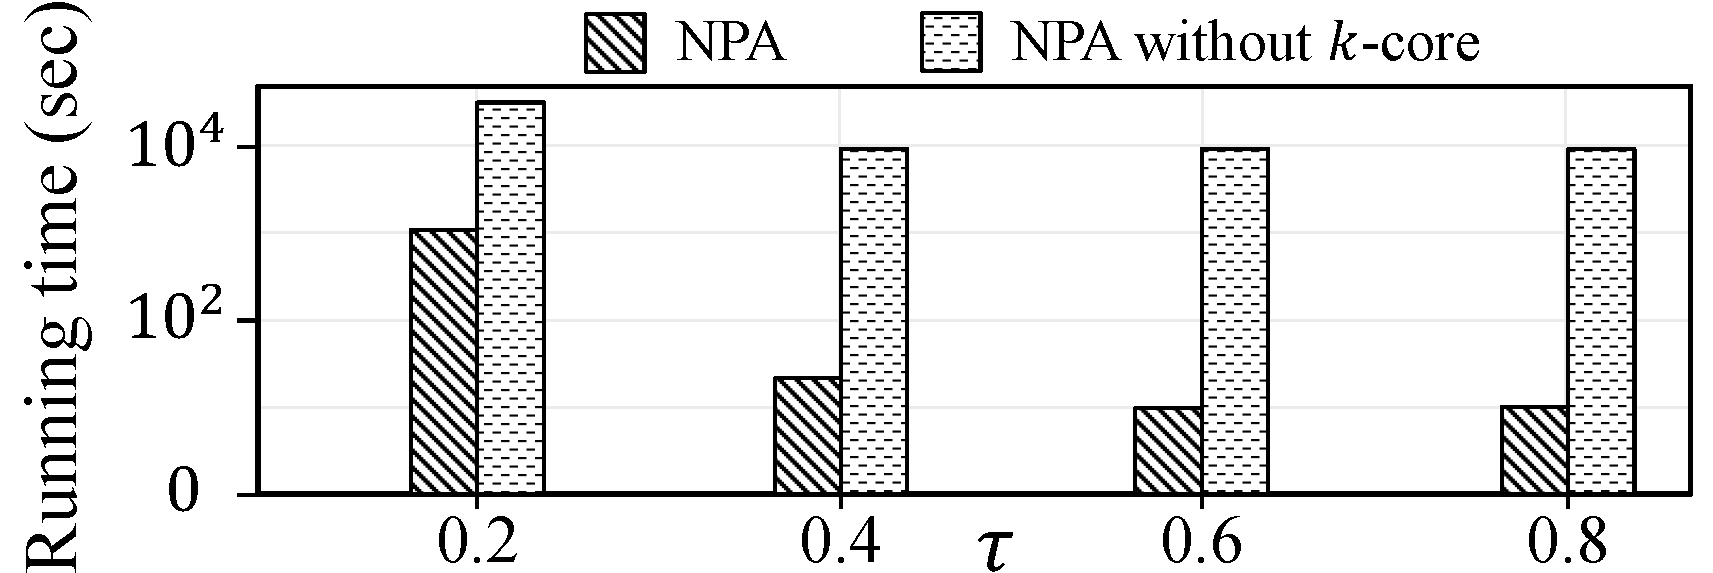
\includegraphics[width=0.8\linewidth]{figures/k_core_effect_thin.pdf}
\vspace{-0.4cm}
\caption{\textbf{EQ4.} Effect on $k$-core (Brightkite)}  
\vspace{-0.3cm}
\label{fig:k_core}
\end{figure}


\spara{\textbf{EQ4. Effect on $k$-core}.} In our algorithm, we use the $k$-core connected component as a first step to find the initial subgraph. We observed the results with and without $k$-core preprocessing. Although the resultant nodes and their sizes were the same in various $\tau$ conditions, as shown in Figure~\ref{fig:k_core}, the running time differed significantly in the Brightkite dataset. This discrepancy is due to the $k$-core preprocessing significantly reducing the size of the initial graph, which decreases the time required to compute non-articulation nodes, a process with a time complexity of $O(|V|+|E|)$.







\section{Conclusion}\label{sec:conclusion}
In this paper, we introduced the {\flexi} problem, a more flexible and generalised classical clique problem, and proposed a non-articulation peeling algorithm (\NPA) to efficiently identify {\flexi} subgraphs in large networks. Our theoretical analysis established the NP-hardness of the maximum {\flexi} problem. Through extensive experiments, we demonstrated the efficiency of our algorithm on both synthetic and real-world datasets. Future work will focus on designing more effective approximation algorithms and considering index-based approach to efficiently retrieve {\flexi} in dynamic networks. 

\bibliographystyle{ACM-Reference-Format}
\bibliography{cikm24}
\end{document}